%&pdflatex
\documentclass[mathserif]{beamer} %, handout
\usetheme[progressbar=foot]{metropolis}
\setbeamertemplate{caption*}[numbered]

\usepackage[utf8x]{inputenc}
\usepackage[T2A]{fontenc}
\usepackage[english,russian]{babel}

\usepackage{amssymb, amsmath, amsfonts, mathtools, mathrsfs}
\usepackage[normalem]{ulem} % for sout
\usepackage{changepage} % for adjustwidth
\usepackage{tabu, tabulary}
\usepackage{comment}

\title{Консервативный проекционный метод решения уравнения Больцмана для неравномерных сеток}
\author{Рогозин Олег Анатольевич}
\institute{
    Вычислительный центр ФИЦ ИУ РАН
}
\date{}

\newcommand{\Kn}{\mathrm{Kn}}
\newcommand{\St}{\mathrm{St}}
\newcommand{\Ma}{\mathrm{Ma}}
\newcommand{\loc}{\mathrm{loc}}
\newcommand{\eqdef}{\overset{\mathrm{def}}{=}}
\newcommand{\dd}{\:\mathrm{d}}
\newcommand{\pder}[2][]{\frac{\partial#1}{\partial#2}}
\newcommand{\pderdual}[2][]{\frac{\partial^2#1}{\partial#2^2}}
\newcommand{\pderder}[3][]{\frac{\partial^2#1}{\partial#2\partial#3}}
\newcommand{\Pder}[2][]{\partial#1/\partial#2}
\newcommand{\dxi}{\boldsymbol{\dd\xi}}
\newcommand{\domega}{\boldsymbol{\dd\omega}}
\newcommand{\bomega}{\boldsymbol{\omega}}
\newcommand{\bxi}{\boldsymbol{\xi}}
\newcommand{\bh}{\boldsymbol{h}}
\newcommand{\be}{\boldsymbol{e}}
\newcommand{\Nu}{\mathcal{N}}
\newcommand{\Mu}{\mathcal{M}}
\newcommand{\OO}[1]{O(#1)}
\newcommand{\Set}[2]{\{\,{#1}:{#2}\,\}}
\newcommand{\xoverbrace}[2][\vphantom{\int}]{\overbrace{#1#2}}
\newcommand{\Cite}[2][]{\alert{\textsc{#2 #1}}}
\newcommand{\inner}[2]{\left\langle{#1},{#2}\right\rangle}

\newcommand\pro{\item[$+$]}
\newcommand\con{\item[$-$]}

% use Russian tradition
\renewcommand{\phi}{\varphi}
\renewcommand{\epsilon}{\varepsilon}

\begin{document}

\frame{\titlepage}

\begin{frame}
    \frametitle{Содержание}
    \linespread{0.8}
    \tableofcontents
\end{frame}

\section{Классификация методов}

\begin{frame}
    \frametitle{Численные методы решения уравнения Больцмана}
    Ключевые свойства:
    \begin{itemize}
        \item сохранение массы, импульса и кинетической энергии;
        \item выполнение \(\mathcal{H}\)-теоремы;
        \item положительность \(f>0\).
    \end{itemize}
\end{frame}

\begin{frame}
    \frametitle{Численные методы решения уравнения Больцмана}
    \setlength{\leftmarginii}{10pt}
    \setlength{\leftmarginiii}{\leftmarginii}
    \begin{adjustwidth}{-2.5em}{-2.5em}
    \centering
    \newcommand{\ColW}{0.35\textwidth}
    \begin{tabular}{>{\centering\arraybackslash}p{\ColW}>{\centering\arraybackslash}p{\ColW}>{\centering\arraybackslash}p{\ColW}}
		\centering\bfseries Прямое статистическое моделирование &
		\centering\bfseries {Методы\\дискретных\\скоростей} &
		{\centering\bfseries Проекционные методы} \\
		\begin{itemize}
            \item метод Бёрда
            \begin{itemize}
                \pro неограниченное пространство скоростей
                \con сильный шум статистический
            \end{itemize}
            \item частицы с весом \(\rightarrow\) редкие события
            \item уменьшение дисперсии \(\rightarrow\) медленные течения
        \end{itemize} &
		\begin{itemize}
            \item прямое интегрирование
            \begin{itemize}
                \pro второй порядок
                \con неконсервативный
            \end{itemize}
            \item дискретный газ
            \begin{itemize}
                \pro консервативный
                \con дробный порядок
            \end{itemize}
            \item \alert{консервативное размазывание столкновительной сферы}
        \end{itemize} &
		\begin{itemize}
            \item Фурье--Галёркина (спектральный)
            \begin{itemize}
                \pro алгоритмы БПФ
                \pro спектральная точность
                \con неконсервативный
                \con явление Гиббса
            \end{itemize}
            \item разрывный Галёркин
            \begin{itemize}
                \pro высокий порядок точности
                \con осложнённый
            \end{itemize}
        \end{itemize} \\
	\end{tabular}
    \end{adjustwidth}
\end{frame}

\begin{frame}
    \frametitle{Консервативное размазывание столкновительной сферы}
    \centering
    {\Large Mетоды дискретных скоростей}\vspace{10pt}

    \Cite[1997]{Palczewski, Schneider, Bobylev}:\\
        сходимость дискретного газа < \(\frac14\) % Пальчевски, Шнайд'ер
    \vspace{10pt}
    \setlength{\leftmarginii}{10pt}
    \setlength{\leftmarginiii}{\leftmarginii}
    \begin{adjustwidth}{-2.5em}{-2.5em}
    \centering
    Computers \& Mathematics with Applications Vol. 35, No. 1-2\\
    (special issue edited by C.~Cercignani \& R.~Illner) % Рейнхард

    \newcommand{\ColW}{0.35\textwidth}
    \begin{tabular}{>{\centering\arraybackslash}p{\ColW}>{\centering\arraybackslash}p{\ColW}>{\centering\arraybackslash}p{\ColW}}
		\centering\bfseries Столкновительный интеграл &
		\centering\bfseries Столкновительная сфера &
		{\centering\bfseries Столкновительная пара} \\
		\Cite[1998]{Buet, Cordier, Degond} &
		\Cite[1998]{Babovsky}, \Cite[2002]{G\"orsch} &
		\Cite[1998]{Tcheremissine} \\
	\end{tabular}
    \end{adjustwidth}
\end{frame}

\section{Метод Черемисина для неравномерных решёток скоростей}

\begin{frame}
    \frametitle{Схема решения уравнения Больцмана}
    \vspace{-5pt}
    \begin{equation}
        \pder[f]{t} + \xi_i\pder[f]{x_i} = J(f,f)
    \end{equation}
    \pause\vspace{-10pt}
    \begin{block}{Симметричная схема расщепления}
        \begin{equation}
            S_{A+B}^{\tau} = S_A^{\tau/2}S_B^{\tau}S_A^{\tau/2} + \OO{\tau^2}
        \end{equation}
        \centering \Cite[1968]{Strang}; \Cite[2001]{Bobylev, Ohwada}
    \end{block}
    \vspace{-10pt}
    \begin{columns}[T]
        \pause
        \begin{column}{5cm}
            \begin{block}{Бесстолкновительное УБ}
                \begin{equation}
                    \pder[f]{t} + \xi_i\pder[f]{x_i} = 0
                \end{equation}
                \vspace{-15pt}
                \begin{itemize}
                    \item метод конечных объёмов
                    \item TVD-схема \(\OO{\tau^2, h^2}\)
                    \item (не)структурированная сетка
                \end{itemize}
            \end{block}
        \end{column}
        \pause
        \begin{column}{6.5cm}
            \begin{block}{Пространственно-однородное УБ}
                \begin{equation}
                    \pder[f]{t} = J(f,f)
                \end{equation}
                \vspace{-15pt}
                \begin{itemize}
                    \item проекционный метод дискретных скоростей
                    \item схема в дробных шагах \(\OO{\tau^2, h^2}\)
                    \item прямоугольная решётка
                \end{itemize}
            \end{block}
        \end{column}
    \end{columns}
\end{frame}

\begin{frame}
    \frametitle{Дискретизация пространства скоростей}
    % Группа для УБ, просто множество для модельных типа БГК
    Решётка \(\mathcal{V} = \Set{\xi_\gamma}{\gamma\in\Gamma}\) построена так, что
    \begin{equation}\label{eq:xi_cubature}
        \int F(\bxi) \dxi \approx \sum_{\gamma\in\Gamma} F_\gamma w_\gamma =
            \sum_{\gamma\in\Gamma} \hat{F_\gamma},
            \quad F_\gamma = F(\bxi_\gamma),
    \end{equation}\vspace{-10pt}

    где \(\sum_{\gamma\in\Gamma} w_\gamma = V_\Gamma\) "--- объём, покрываемый скоростной решёткой.
    \pause\vspace{10pt}

    Симметризированный интеграл столкновений\vspace{-20pt}

    \begin{equation}\label{eq:symm_ci}
        J(f_\gamma, f_\gamma) = \frac14\int \left(
            \delta_\gamma + \delta_{\gamma*} - \delta'_\gamma - \delta'_{\gamma*}
        \right) (f'f'_* - ff_*)B \dd\Omega(\boldsymbol{\alpha}) \dxi\dxi_*
    \end{equation}\vspace{-30pt}

    имеет следующий дискретный аналог:
    \begin{equation}\label{eq:discrete_symm_ci}
        \footnotesize
        \hat{J}_\gamma = \frac{\pi V_\Gamma^2}{\displaystyle\sum_{\nu\in\Nu} w_{\nu}w_{*\nu}}
            \sum_{\nu\in\Nu} \bigg(
                \delta_{\gamma\nu} + \delta_{*\gamma\nu} -
                \xoverbrace{ \alert{\delta'_{\gamma\nu}} - \alert{\delta'_{*\gamma\nu}} }^\text{projection}
            \bigg)\bigg(
                \xoverbrace{ \frac{w_{\nu}w_{*\nu}}{\alert{w'_{\nu}w'_{*\nu}}}
                \alert{\hat{f}'_{\nu}\hat{f}'_{*\nu}} }^\text{interpolation} - \hat{f}_{\nu}\hat{f}_{*\nu}
            \bigg)B_\nu.
    \end{equation}\vspace{-10pt}
\end{frame}

\begin{frame}
    \frametitle{Консервативное проецирование}
    \centering{\Large\bf Почему метод называется <<проекционным>>?}
    \vspace{10pt}

    Проекционная процедура Петрова"--~Галёркина:
    \begin{equation}\label{eq:Petrov-Galerkin}
        \int \xoverbrace{ \psi_s(\bxi_\gamma) }^\text{test space} \bigg(
            \alert{\delta(\bxi'-\bxi_\gamma)} - \sum_{a\in\Lambda} r_{\lambda,a}
            \xoverbrace{ \delta(\bxi_{\lambda+s_a}-\bxi_\gamma) }^\text{trial space}
        \bigg) \dxi_\gamma = 0.
    \end{equation}
    \begin{itemize}
        \item \(r_{\lambda,a}\) "--- проекционные веса (в пространстве \(\mathcal{V}\))
        \item \(\mathcal{S} = \Set{s_a}{a\in\Lambda, r_{\lambda,a}\neq0}\) "--- проекционный шаблон \\(набор правил смещения)
        \item \(\psi_0 = 1, \psi_i = \xi_i, \psi_4 = \xi_i^2\) "--- столкновительные инварианты
        \item всё то же справедливо \(\alert{\delta(\bxi'_*-\bxi_\gamma)}\)
    \end{itemize}
\end{frame}

\begin{frame}
    \frametitle{Интерполирование функции распределения}
    Среднее взвешенное по Колмогорову:
    \begin{equation}\label{eq:Kolmogorov_mean}
        \begin{dcases}
            \alert{\hat{f}'_{\nu}} = \phi^{-1}_f\left(\sum_{a\in\Lambda} q_{\lambda,a}
                \phi_f\left(\hat{f}_{\lambda+s_a}\right)\right), \\
            \alert{w'_{\nu}} = \phi^{-1}_w\left(\sum_{a\in\Lambda} p_{\lambda,a}
                \phi_w\left(w_{\lambda+s_a}\right)\right), \\
        \end{dcases}
    \end{equation}
    Если взять геометрическое среднее
    \begin{equation}\label{eq:geometric_mean}
       \phi_{f,w}(x) = \ln(x), \quad \phi_{f,w}^{-1}(x) = \exp(x), \quad p_{\lambda,a} = q_{\lambda,a} = r_{\lambda,a},
    \end{equation}
    то выполняется \(\mathcal{H}\)-теорема и
    \begin{equation}\label{eq:strict_interpolation}
        \hat{J}_\gamma(\hat{f}_{M\gamma}, \hat{f}_{M\gamma}) = 0.
    \end{equation}
    То же самое справедливо для \(\alert{w'_{*\nu}}\) и \(\alert{\hat{f}'_{*\nu}}\).
\end{frame}

\begin{frame}
    \frametitle{Пространственно-однородная задача Коши}
    Перепишем
    \begin{equation}
        \hat{J}_\gamma = \frac{\pi V_\Gamma^2}{\sum_{\nu\in\Nu} w_{\nu}w_{*\nu}}
        \sum_{\nu\in\Nu} \left(
            \delta_{\gamma\nu} + \delta_{*\gamma\nu} -
            \delta'_{\gamma\nu} - \delta'_{*\gamma\nu}
        \right)\big(\cdots\big)B_\nu
    \end{equation}
    как
    \begin{equation}
        \hat{J}_{\gamma} = \sum_{j=1}^N \hat{\Delta}_{\gamma}^{n+(j-1)/N}, \quad N=|\Nu|.
    \end{equation}
    Тогда можно построить консервативную схему в дробных шагах
    \begin{equation}\label{eq:fractional_step_scheme}
        \hat{f}_\gamma^{n+j/N} = \hat{f}_\gamma^{n+(j-1)/N} + \frac{\tau}{N}\hat{\Delta}_{\gamma}^{n+(j-1)/N}
        \quad (j = 1,\dotsc,N).
    \end{equation}
    \pause % микроскопическая консервативность
    \begin{itemize}
        \item каждый \(\hat{\Delta}_{\gamma}^{n+(j-1)/N}\) содержит \(2(1+|\mathcal{S}|)\) ненулевых элементов
        \item каждый дробный шаг сохраняет массу, импульс, энергию и не уменьшает энтропию
    \end{itemize}
\end{frame}

\begin{frame}
    \frametitle{Положительность функции распределения}
    Оценки на \(N\), гарантирующие \(\hat{f}_\gamma^{n+j/N}>0\):
    \begin{gather*}
        N > A \hat{f}_{\max}\epsilon_w^2 \alert{\max_{\substack{s_a,s_b\in\mathcal{S}\\\gamma\in\Gamma}}
            \frac{\hat{f}_{\gamma+s_a}}{\hat{f}_{\gamma+s_b}}} , \quad r_{\gamma,a} > 0, \\
        N > A \hat{f}_{\max} \bar{r}_{\max} \alert{\max_{\gamma,\sigma\in\Gamma}\frac{\hat{f_\gamma}}{\hat{f_\sigma}}}, \quad
            \bar{r}_{\max} = \max_{\gamma\in\Gamma,a\in\Lambda}( -r_{\gamma,a} ).
    \end{gather*}
    \begin{gather*}
        \footnotesize
        A = \frac{\pi\tau V_\Gamma^2 N B_{\max}}{\sum_{\nu\in\Nu} w_{\nu}w_{*\nu}}, \quad
        B_{\max} = \max_{\substack{\gamma,\sigma\in\Gamma\\\boldsymbol{\alpha}\in S^2}}
            B(\boldsymbol{\alpha}, \bxi_{\gamma}, \bxi_{\sigma}) = \OO{\xi_{\max}}, \\
        \xi_{\max} = \max_{\gamma\in\Gamma}|\bxi_\gamma|, \quad
        \hat{f}_{\max} = \max_{\gamma\in\Gamma} \hat{f}_\gamma, \quad
        \epsilon_w = \max_{\gamma,\sigma\in\Gamma} \frac{w_\gamma}{w_\sigma}.
    \end{gather*}
    \pause
    На равномерной решётке
    \begin{itemize}
        \item \(\bar{r}_{\max}=1/8\) для \(\mathcal{S}=5\), \(\mathcal{S}=7\)
        \item \(\bar{r}_{\max}=1/16\) для \(\mathcal{S}=13\)
    \end{itemize}
\end{frame}

\begin{frame}
    \frametitle{Положительность функции распределения}
    На практике
    \begin{equation}
        \hat{J}_\gamma = \sum_{\nu\in\Nu\alert{\setminus\Mu}} \hat{\Delta}_{\gamma\nu},
    \end{equation}
    где \(\alert{\Mu}\) "--- множество кубатурных точек, нарушающих позитивность.
    \vspace{20pt}\pause

    Достаточно поддерживать малость
    \begin{equation}
        \frac{\pi V_\Gamma^2}{\rho\sum_{\nu\in\Nu} w_{\nu}w_{*\nu}}
        \sum_{\nu\in\alert{\Mu}} \left|
            \hat{f}_{\lambda_\nu}\hat{f}_{\mu_\nu} - \hat{f}_{\nu}\hat{f}_{*\nu}
        \right|B_\nu < \epsilon.
    \end{equation}
    Обычно \(\epsilon \lesssim 10^{-5}\).
\end{frame}

\section{Нелинейное течение Куэтта}

\begin{frame}
    \frametitle{Функция распределения \(\Delta{v}=2\), срез \(\xi_z=0.1665\)}
    \vspace{-20pt} \[ Kn=0.1 \] \vspace{-20pt}
    \begin{columns}
        \column{.55\textwidth}
        \begin{figure}
            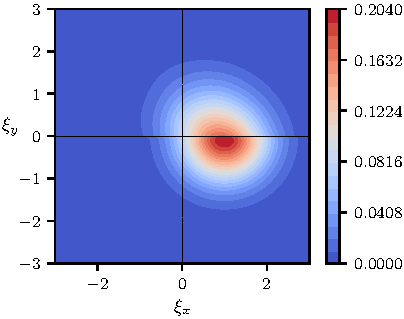
\includegraphics[width=\linewidth]{{{couette/kn0.1-boundary}}}
            \caption{Возле границы \(y=0.4990\)}
        \end{figure}
        \column{.55\textwidth}
        \begin{figure}
            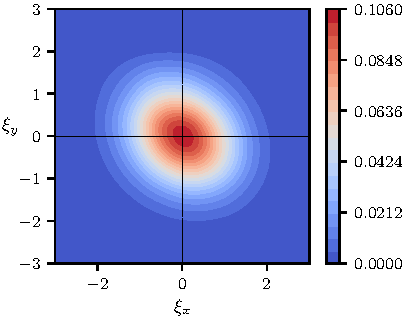
\includegraphics[width=\linewidth]{{{couette/kn0.1-center}}}
            \caption{Вблизи центра \(y=0.0082\)}
        \end{figure}
    \end{columns}
\end{frame}

\begin{frame}
    \frametitle{Функция распределения \(\Delta{v}=2\), срез \(\xi_z=0.1665\)}
    \vspace{-20pt} \[ Kn=1 \] \vspace{-20pt}
    \begin{columns}
        \column{.55\textwidth}
        \begin{figure}
            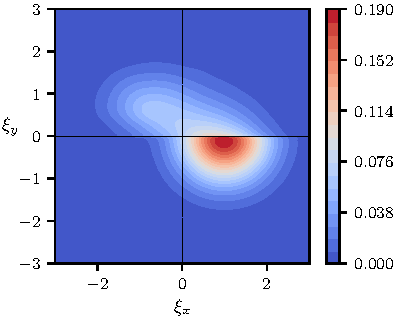
\includegraphics[width=\linewidth]{{{couette/kn1.0-boundary}}}
            \caption{Возле границы \(y=0.4929\)}
        \end{figure}
        \column{.55\textwidth}
        \begin{figure}
            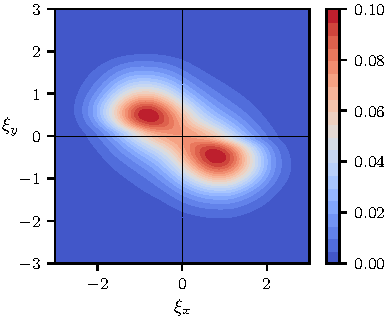
\includegraphics[width=\linewidth]{{{couette/kn1.0-center}}}
            \caption{Вблизи центра \(y=0.0083\)}
        \end{figure}
    \end{columns}
\end{frame}

\begin{frame}
    \frametitle{Функция распределения \(\Delta{v}=2\), срез \(\xi_z=0.1665\)}
    \vspace{-20pt} \[ Kn=10 \] \vspace{-20pt}
    \begin{columns}
        \column{.55\textwidth}
        \begin{figure}
            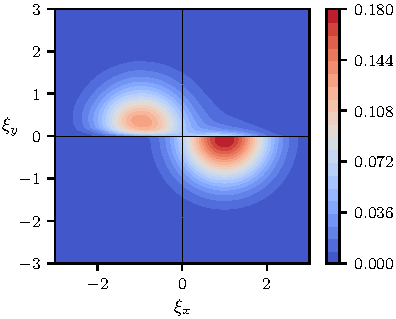
\includegraphics[width=\linewidth]{{{couette/kn10-boundary}}}
            \caption{Возле границы \(y=0.4917\)}
        \end{figure}
        \column{.55\textwidth}
        \begin{figure}
            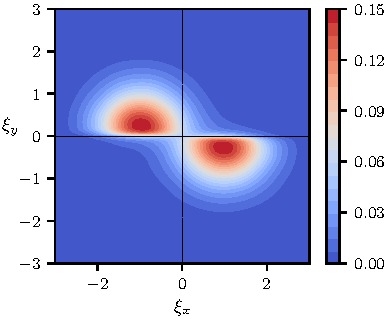
\includegraphics[width=\linewidth]{{{couette/kn10-center}}}
            \caption{Вблизи центра \(y=0.0083\)}
        \end{figure}
    \end{columns}
\end{frame}

\begin{frame}
    \frametitle{Логарифмические сингулярности}
    \begin{itemize}
        \item \Cite[2014]{Chen, Liu, Takata}
        \[ \pder[f]{x_i}n_i = \frac{C}{\Kn}\ln\frac{(x_i-x_{Bi})n_i}{\Kn} + \OO{1}. \]
        \item \Cite[2016]{Chen, Funagane, Liu, Takata}
        \[ \pder[f]{\xi_i}n_i = C\ln\xi_in_i + \OO{1}. \]
    \end{itemize}
    где \(x_{Bi}\) "--- координата граничной поверхности.
\end{frame}

\begin{frame}
    \frametitle{Профили сдвигового напряжения}
    \[ p_{xy} = -\Gamma_1(T_H)\pder[v_H]{y}k + \OO{k^3} \]
    \centering
    \includegraphics[width=0.9\linewidth]{couette/Pxy}
\end{frame}

\begin{frame}
    \frametitle{Профили продольной скорости}
    \vspace{-5pt}
    \[ v_x = v_H - \frac{Y_0^--Y_0^+}{p_H}\left(T_H\pder[v_H]{y}\right)_{y=\frac12}k + \OO{k^2} \]
    \vspace{-5pt}
    \centering
    \includegraphics[width=0.9\linewidth]{couette/vx}
\end{frame}

\begin{frame}
    \frametitle{Профили температуры}
    \vspace{-5pt}
    \[ T = T_H - \frac{\Theta_1^-+\Theta_1^+}{p_H}\left(T_H\pder[T_H]{y}\right)_{y=\frac12}k + \OO{k^2} \]
    \vspace{-5pt}
    \centering
    \includegraphics[width=0.9\linewidth]{couette/tau}
\end{frame}

\begin{frame}
    \frametitle{Профили поперечного теплового потока}
    \[ q_y = -\frac54\Gamma_2(T_H)\pder[T_H]{y}k + q_{yK2}k^2 + \OO{k^3} \]
    \centering
    \includegraphics[width=0.9\linewidth]{couette/qy}
\end{frame}

\begin{frame}
    \frametitle{Профили продольного теплового потока}
    \vspace{-10pt}
    \[ q_x = q_{xK1}k
        + \frac{T_H}{p_H}\left( \frac{\Gamma_3}2 \pderdual[v_H]{y}
            + 4\Gamma_{10} \pder[T_H]{y}\pder[v_H]{y} \right)k^2
        + q_{xK2}k^2 + \OO{k^3} \]
    \vspace{-10pt}
    \centering
    \includegraphics[width=0.9\linewidth]{couette/qx}
\end{frame}

\begin{frame}
    \frametitle{Профили \(P_{xx}-P{yy}\)}
    \vspace{-15pt}
    \[ P_{xxH}-P_{yyH} = \left[ 2\Gamma_9 \left(\pder[v_H]{y}\right)^2
        - \Gamma_3 \pderdual[T_H]{y}
        - \Gamma_7\left(\pder[T_H]{y}\right)^2 \right]\frac{k^2}{p_H} + \OO{k^3} \]
    \vspace{-15pt}
    \centering
    \includegraphics[width=0.9\linewidth]{couette/Pxx}
\end{frame}

\begin{frame}
    \frametitle{Профили \(P_{zz}-P{yy}\)}
    \footnotesize
    \vspace{-15pt}
    \[ P_{zzH}-P_{yyH} = \left[ 2(\Gamma_9-\Gamma_8) \left(\pder[v_H]{y}\right)^2
        - \Gamma_3 \pderdual[T_H]{y}
        - \Gamma_7\left(\pder[T_H]{y}\right)^2 \right]\frac{k^2}{p_H} + \OO{k^3} \]
    \vspace{-15pt}
    \centering
    \includegraphics[width=0.9\linewidth]{couette/Pzz}
\end{frame}

\begin{frame}
    \frametitle{Транспортные коэффициенты для модели твёрдых сфер}
    \begin{alignat*}{2}
        \gamma_1 &= 1.270042427, \quad &\text{\Cite[1957]{Pekeris, Alterman}} \\
        \gamma_2 &= 1.922284065, \quad &\text{\Cite[1957]{Pekeris, Alterman}} \\
        \gamma_3 &= 1.947906335, \quad &\text{\Cite[1992]{Ohwada, Sone}} \\
        \gamma_7 &= 0.189200,    \quad &\text{\Cite[1996]{\footnotesize Sone, Aoki, Takata, Sugimoto, Bobylev}} \\
        \gamma_8 &= 1.495941968, \quad &\text{\Cite[2016]{Rogozin}} \\
        \gamma_9 &= 1.636073458, \quad &\text{\Cite[2016]{Rogozin}} \\
        \gamma_{10} &= 2.4497795.\quad &\text{\Cite[2016]{Rogozin}}
    \end{alignat*}
\end{frame}

\begin{frame}
    \frametitle{Зависимость сдвигового напряжения от \(\Kn\)}
    \vspace{-2pt}
    \centering\hspace{-1.5cm}
    \includegraphics[width=1.1\linewidth]{couette2/shear}
    \hspace{-1.5cm}
\end{frame}

\begin{frame}
    \frametitle{Зависимость продольной скорости от \(\Kn\)}
    \vspace{-2pt}
    \centering\hspace{-1.5cm}
    \includegraphics[width=1.1\linewidth]{couette2/flow}
    \hspace{-1.5cm}
\end{frame}

\begin{frame}
    \frametitle{Зависимость продольного теплового потока от \(\Kn\)}
    \vspace{-2pt}
    \centering\hspace{-1.5cm}
    \includegraphics[width=1.1\linewidth]{couette2/qflow}
    \hspace{-1.5cm}
\end{frame}

\begin{frame}
    \frametitle{Зависимость поперечного теплового потока от \(\Kn\)}
    \vspace{-2pt}
    \centering\hspace{-1.5cm}
    \includegraphics[width=1.1\linewidth]{couette2/qflowy}
    \hspace{-1.5cm}
\end{frame}

\begin{frame}
    \frametitle{Зависимость \(P_{zz}-P_{yy}\) от \(\Kn\)}
    \vspace{-2pt}
    \centering\hspace{-1.5cm}
    \includegraphics[width=1.1\linewidth]{couette2/pzz}
    \hspace{-1.5cm}
\end{frame}

\begin{frame}
    \frametitle{Заключение}
    \begin{itemize}
        \item Удаётся детально разрешить плоские кинетические слои,
        но можно моделировать гиперзвуковые течения с большим перепадом температур.
        \item Вопрос сходимости, особенно влияния проекционного шаблона
        и отрицательных проекционных весов на её скорость.
        \item Нелинейная асимптотическая теория "--- хороший инструмент для верификации
        численных методов.
    \end{itemize}
\end{frame}

\end{document}
